
%% bare_conf.tex
%% V1.4a
%% 2014/09/17
%% by Michael Shell
%% See:
%% http://www.michaelshell.org/
%% for current contact information.
%%
%% This is a skeleton file demonstrating the use of IEEEtran.cls
%% (requires IEEEtran.cls version 1.8a or later) with an IEEE
%% conference paper.
%%
%% Support sites:
%% http://www.michaelshell.org/tex/ieeetran/
%% http://www.ctan.org/tex-archive/macros/latex/contrib/IEEEtran/
%% and
%% http://www.ieee.org/

%%*************************************************************************
%% Legal Notice:
%% This code is offered as-is without any warranty either expressed or
%% implied; without even the implied warranty of MERCHANTABILITY or
%% FITNESS FOR A PARTICULAR PURPOSE! 
%% User assumes all risk.
%% In no event shall IEEE or any contributor to this code be liable for
%% any damages or losses, including, but not limited to, incidental,
%% consequential, or any other damages, resulting from the use or misuse
%% of any information contained here.
%%
%% All comments are the opinions of their respective authors and are not
%% necessarily endorsed by the IEEE.
%%
%% This work is distributed under the LaTeX Project Public License (LPPL)
%% ( http://www.latex-project.org/ ) version 1.3, and may be freely used,
%% distributed and modified. A copy of the LPPL, version 1.3, is included
%% in the base LaTeX documentation of all distributions of LaTeX released
%% 2003/12/01 or later.
%% Retain all contribution notices and credits.
%% ** Modified files should be clearly indicated as such, including  **
%% ** renaming them and changing author support contact information. **
%%
%% File list of work: IEEEtran.cls, IEEEtran_HOWTO.pdf, bare_adv.tex,
%%                    bare_conf.tex, bare_jrnl.tex, bare_conf_compsoc.tex,
%%                    bare_jrnl_compsoc.tex, bare_jrnl_transmag.tex
%%*************************************************************************


% *** Authors should verify (and, if needed, correct) their LaTeX system  ***
% *** with the testflow diagnostic prior to trusting their LaTeX platform ***
% *** with production work. IEEE's font choices and paper sizes can       ***
% *** trigger bugs that do not appear when using other class files.       ***                          ***
% The testflow support page is at:
% http://www.michaelshell.org/tex/testflow/



\documentclass[conference]{IEEEtran}
% Some Computer Society conferences also require the compsoc mode option,
% but others use the standard conference format.
%
% If IEEEtran.cls has not been installed into the LaTeX system files,
% manually specify the path to it like:
% \documentclass[conference]{../sty/IEEEtran}





% Some very useful LaTeX packages include:
% (uncomment the ones you want to load)


% *** MISC UTILITY PACKAGES ***
%
%\usepackage{ifpdf}
% Heiko Oberdiek's ifpdf.sty is very useful if you need conditional
% compilation based on whether the output is pdf or dvi.
% usage:
% \ifpdf
%   % pdf code
% \else
%   % dvi code
% \fi
% The latest version of ifpdf.sty can be obtained from:
% http://www.ctan.org/tex-archive/macros/latex/contrib/oberdiek/
% Also, note that IEEEtran.cls V1.7 and later provides a builtin
% \ifCLASSINFOpdf conditional that works the same way.
% When switching from latex to pdflatex and vice-versa, the compiler may
% have to be run twice to clear warning/error messages.






% *** CITATION PACKAGES ***
%
%\usepackage{cite}
% cite.sty was written by Donald Arseneau
% V1.6 and later of IEEEtran pre-defines the format of the cite.sty package
% \cite{} output to follow that of IEEE. Loading the cite package will
% result in citation numbers being automatically sorted and properly
% "compressed/ranged". e.g., [1], [9], [2], [7], [5], [6] without using
% cite.sty will become [1], [2], [5]--[7], [9] using cite.sty. cite.sty's
% \cite will automatically add leading space, if needed. Use cite.sty's
% noadjust option (cite.sty V3.8 and later) if you want to turn this off
% such as if a citation ever needs to be enclosed in parenthesis.
% cite.sty is already installed on most LaTeX systems. Be sure and use
% version 5.0 (2009-03-20) and later if using hyperref.sty.
% The latest version can be obtained at:
% http://www.ctan.org/tex-archive/macros/latex/contrib/cite/
% The documentation is contained in the cite.sty file itself.






% *** GRAPHICS RELATED PACKAGES ***
%
\ifCLASSINFOpdf
  % \usepackage[pdftex]{graphicx}
  % declare the path(s) where your graphic files are
  % \graphicspath{{../pdf/}{../jpeg/}}
  % and their extensions so you won't have to specify these with
  % every instance of \includegraphics
  % \DeclareGraphicsExtensions{.pdf,.jpeg,.png}
\else
  % or other class option (dvipsone, dvipdf, if not using dvips). graphicx
  % will default to the driver specified in the system graphics.cfg if no
  % driver is specified.
  % \usepackage[dvips]{graphicx}
  % declare the path(s) where your graphic files are
  % \graphicspath{{../eps/}}
  % and their extensions so you won't have to specify these with
  % every instance of \includegraphics
  % \DeclareGraphicsExtensions{.eps}
\fi
% graphicx was written by David Carlisle and Sebastian Rahtz. It is
% required if you want graphics, photos, etc. graphicx.sty is already
% installed on most LaTeX systems. The latest version and documentation
% can be obtained at: 
% http://www.ctan.org/tex-archive/macros/latex/required/graphics/
% Another good source of documentation is "Using Imported Graphics in
% LaTeX2e" by Keith Reckdahl which can be found at:
% http://www.ctan.org/tex-archive/info/epslatex/
%
% latex, and pdflatex in dvi mode, support graphics in encapsulated
% postscript (.eps) format. pdflatex in pdf mode supports graphics
% in .pdf, .jpeg, .png and .mps (metapost) formats. Users should ensure
% that all non-photo figures use a vector format (.eps, .pdf, .mps) and
% not a bitmapped formats (.jpeg, .png). IEEE frowns on bitmapped formats
% which can result in "jaggedy"/blurry rendering of lines and letters as
% well as large increases in file sizes.
%
% You can find documentation about the pdfTeX application at:
% http://www.tug.org/applications/pdftex





% *** MATH PACKAGES ***
%
%\usepackage[cmex10]{amsmath}
% A popular package from the American Mathematical Society that provides
% many useful and powerful commands for dealing with mathematics. If using
% it, be sure to load this package with the cmex10 option to ensure that
% only type 1 fonts will utilized at all point sizes. Without this option,
% it is possible that some math symbols, particularly those within
% footnotes, will be rendered in bitmap form which will result in a
% document that can not be IEEE Xplore compliant!
%
% Also, note that the amsmath package sets \interdisplaylinepenalty to 10000
% thus preventing page breaks from occurring within multiline equations. Use:
%\interdisplaylinepenalty=2500
% after loading amsmath to restore such page breaks as IEEEtran.cls normally
% does. amsmath.sty is already installed on most LaTeX systems. The latest
% version and documentation can be obtained at:
% http://www.ctan.org/tex-archive/macros/latex/required/amslatex/math/





% *** SPECIALIZED LIST PACKAGES ***
%
%\usepackage{algorithmic}
% algorithmic.sty was written by Peter Williams and Rogerio Brito.
% This package provides an algorithmic environment fo describing algorithms.
% You can use the algorithmic environment in-text or within a figure
% environment to provide for a floating algorithm. Do NOT use the algorithm
% floating environment provided by algorithm.sty (by the same authors) or
% algorithm2e.sty (by Christophe Fiorio) as IEEE does not use dedicated
% algorithm float types and packages that provide these will not provide
% correct IEEE style captions. The latest version and documentation of
% algorithmic.sty can be obtained at:
% http://www.ctan.org/tex-archive/macros/latex/contrib/algorithms/
% There is also a support site at:
% http://algorithms.berlios.de/index.html
% Also of interest may be the (relatively newer and more customizable)
% algorithmicx.sty package by Szasz Janos:
% http://www.ctan.org/tex-archive/macros/latex/contrib/algorithmicx/




% *** ALIGNMENT PACKAGES ***
%
%\usepackage{array}
% Frank Mittelbach's and David Carlisle's array.sty patches and improves
% the standard LaTeX2e array and tabular environments to provide better
% appearance and additional user controls. As the default LaTeX2e table
% generation code is lacking to the point of almost being broken with
% respect to the quality of the end results, all users are strongly
% advised to use an enhanced (at the very least that provided by array.sty)
% set of table tools. array.sty is already installed on most systems. The
% latest version and documentation can be obtained at:
% http://www.ctan.org/tex-archive/macros/latex/required/tools/


% IEEEtran contains the IEEEeqnarray family of commands that can be used to
% generate multiline equations as well as matrices, tables, etc., of high
% quality.




% *** SUBFIGURE PACKAGES ***
%\ifCLASSOPTIONcompsoc
%  \usepackage[caption=false,font=normalsize,labelfont=sf,textfont=sf]{subfig}
%\else
%  \usepackage[caption=false,font=footnotesize]{subfig}
%\fi
% subfig.sty, written by Steven Douglas Cochran, is the modern replacement
% for subfigure.sty, the latter of which is no longer maintained and is
% incompatible with some LaTeX packages including fixltx2e. However,
% subfig.sty requires and automatically loads Axel Sommerfeldt's caption.sty
% which will override IEEEtran.cls' handling of captions and this will result
% in non-IEEE style figure/table captions. To prevent this problem, be sure
% and invoke subfig.sty's "caption=false" package option (available since
% subfig.sty version 1.3, 2005/06/28) as this is will preserve IEEEtran.cls
% handling of captions.
% Note that the Computer Society format requires a larger sans serif font
% than the serif footnote size font used in traditional IEEE formatting
% and thus the need to invoke different subfig.sty package options depending
% on whether compsoc mode has been enabled.
%
% The latest version and documentation of subfig.sty can be obtained at:
% http://www.ctan.org/tex-archive/macros/latex/contrib/subfig/




% *** FLOAT PACKAGES ***
%
%\usepackage{fixltx2e}
% fixltx2e, the successor to the earlier fix2col.sty, was written by
% Frank Mittelbach and David Carlisle. This package corrects a few problems
% in the LaTeX2e kernel, the most notable of which is that in current
% LaTeX2e releases, the ordering of single and double column floats is not
% guaranteed to be preserved. Thus, an unpatched LaTeX2e can allow a
% single column figure to be placed prior to an earlier double column
% figure. The latest version and documentation can be found at:
% http://www.ctan.org/tex-archive/macros/latex/base/


%\usepackage{stfloats}
% stfloats.sty was written by Sigitas Tolusis. This package gives LaTeX2e
% the ability to do double column floats at the bottom of the page as well
% as the top. (e.g., "\begin{figure*}[!b]" is not normally possible in
% LaTeX2e). It also provides a command:
%\fnbelowfloat
% to enable the placement of footnotes below bottom floats (the standard
% LaTeX2e kernel puts them above bottom floats). This is an invasive package
% which rewrites many portions of the LaTeX2e float routines. It may not work
% with other packages that modify the LaTeX2e float routines. The latest
% version and documentation can be obtained at:
% http://www.ctan.org/tex-archive/macros/latex/contrib/sttools/
% Do not use the stfloats baselinefloat ability as IEEE does not allow
% \baselineskip to stretch. Authors submitting work to the IEEE should note
% that IEEE rarely uses double column equations and that authors should try
% to avoid such use. Do not be tempted to use the cuted.sty or midfloat.sty
% packages (also by Sigitas Tolusis) as IEEE does not format its papers in
% such ways.
% Do not attempt to use stfloats with fixltx2e as they are incompatible.
% Instead, use Morten Hogholm'a dblfloatfix which combines the features
% of both fixltx2e and stfloats:
%
% \usepac_jage{dblfloatfix}
% The latest version can be found at:
% http://www.ctan.org/tex-archive/macros/latex/contrib/dblfloatfix/




% *** PDF, URL AND HYPERLINK PACKAGES ***
%
%\usepackage{url}
% url.sty was written by Donald Arseneau. It provides better support for
% handling and breaking URLs. url.sty is already installed on most LaTeX
% systems. The latest version and documentation can be obtained at:
% http://www.ctan.org/tex-archive/macros/latex/contrib/url/
% Basically, \url{my_url_here}.




% *** Do not adjust lengths that control margins, column widths, etc. ***
% *** Do not use packages that alter fonts (such as pslatex).         ***
% There should be no need to do such things with IEEEtran.cls V1.6 and later.
% (Unless specifically asked to do so by the journal or conference you plan
% to submit to, of course. )


% correct bad hyphenation here
\hyphenation{op-tical net-works semi-conduc-tor}
\usepackage{cite,times,amsmath,epsfig,algorithmic,array}
\usepackage{mdwmath}
\usepackage{mdwtab}
\usepackage{eqparbox}
%\usepackage{psfig}
\usepackage{cite}
\usepackage{graphicx}
\usepackage{amsfonts}
%\usepackage{intmacros}
\usepackage{epstopdf}
\usepackage{amsfonts}
\usepackage{amsmath}
\usepackage{amssymb}
\usepackage{amsthm}
\usepackage{algorithm}
\usepackage{algorithmic}


\begin{document}
%
% paper title
% Titles are generally capitalized except for words such as a, an, and, as,
% at, but, by, for, in, nor, of, on, or, the, to and up, which are usually
% not capitalized unless they are the first or last word of the title.
% Linebreaks \\ can be used within to get better formatting as desired.
% Do not put math or special symbols in the title.
\title{Assisted Transmission for Secure Communication}


% author names and affiliations
% use a multiple column layout for up to three different
% affiliations
\author{
\IEEEauthorblockN{Yanqing Liu, Liang Dong and Robert J. Marks II}
\IEEEauthorblockA{Department of Electrical and Computer Engineering\\
Baylor University, Waco, Texas \\
Email: \{yanqing\_liu, liang\_dong, robert\_marks\}@baylor.edu}
}

% conference papers do not typically use \thanks and this command
% is locked out in conference mode. If really needed, such as for
% the acknowledgment of grants, issue a \IEEEoverridecommandlockouts
% after \documentclass

% for over three affiliations, or if they all won't fit within the width
% of the page, use this alternative format:
% 
%\author{\IEEEauthorblockN{Michael Shell\IEEEauthorrefmark{1},
%Homer Simpson\IEEEauthorrefmark{2},
%James Kirk\IEEEauthorrefmark{3}, 
%Montgomery Scott\IEEEauthorrefmark{3} and
%Eldon Tyrell\IEEEauthorrefmark{4}}
%\IEEEauthorblockA{\IEEEauthorrefmark{1}School of Electrical and Computer Engineering\\
%Georgia Institute of Technology,
%Atlanta, Georgia 30332--0250\\ Email: see http://www.michaelshell.org/contact.html}
%\IEEEauthorblockA{\IEEEauthorrefmark{2}Twentieth Century Fox, Springfield, USA\\
%Email: homer@thesimpsons.com}
%\IEEEauthorblockA{\IEEEauthorrefmark{3}Starfleet Academy, San Francisco, California 96678-2391\\
%Telephone: (800) 555--1212, Fax: (888) 555--1212}
%\IEEEauthorblockA{\IEEEauthorrefmark{4}Tyrell Inc., 123 Replicant Street, Los Angeles, California 90210--4321}}




% use for special paper notices
%\IEEEspecialpapernotice{(Invited Paper)}




% make the title area
\maketitle

% As a general rule, do not put math, special symbols or citations
% in the abstract
\begin{abstract}
A communication network is considered that consists of several transmitters, a receiver and an eavesdropper.  When one transmitter establishes secure communication with the receiver, the other transmitters act as helpers to send noise to confuse the eavesdropper.  The transmitter and the helpers are equipped with multiple antennas while the legitimate receiver or the eavesdropper has one antenna.  The transmitter and the helpers know the channels toward the receiver.  The channels toward the eavesdropper are partially known and modeled with uncertainty ellipsoids.  The transmitter applies maximum ratio transmission to the legitimate receiver.  The helpers send noise to guarantee the secrecy rate requirement.  Based on robust programming, a centralized optimization problem is developed for the helpers to transmit noise effectively with minimum total transmit power.  Furthermore, a distributed algorithm is developed which scales well with a large number of helpers. 
\end{abstract}

% no keywords




% For peer review papers, you can put extra information on the cover
% page as needed:
% \ifCLASSOPTIONpeerreview
% \begin{center} \bfseries EDICS Category: 3-BBND \end{center}
% \fi
%
% For peerreview papers, this IEEEtran command inserts a page break and
% creates the second title. It will be ignored for other modes.
\IEEEpeerreviewmaketitle



\section{Introduction}
% no \IEEEPARstart

% You must have at least 2 lines in the paragraph with the drop letter
% (should never be an issue)
In wireless communication, security is a major concern due to the broadcast nature of wireless channel. Instead of cryptography method such as encryption, physical layer security has attracted a lot of research attention.

One kind of the physical layer security methods is using artificial noise to degrade the performance of the eavesdropper. Many researchers investigated the case where the transmitter allocates part of the transmit power to send artificial noise and optimize the power allocation. S. H. Chae \emph{et al.} assumed there is a secrecy protected zone. The additional secrecy enhancement is realized using artificial noise and optimal power allocation between the information-bearing signal and artificial noise is derived \cite{chae2014enhanced}.  P.-H. Lin \emph{et al.} assumed perfect legitimate channel state information but only the statistics of the eavesdropper's channel. A generalized artificial noise scheme which allows the injection of the artificial noise to the legitimate channel was proposed \cite{lin2013secrecy}. H. Qin \emph{et al.} considered the discrete channel inputs, and investigated the power allocation and artificial noise design for OFDM wiretap channels \cite{qin2013power}. summarize the methods of cooperative jamming \cite{cooperative_jamming}.

The cooperation among the transmitting nodes to improve the secrecy capacity is investigated. E. Tekin \emph{et al.} showed that cooperation among users is helpful for achieving secrecy. Cooperative jamming was proposed,  where some users are prevented from transmitting message and "jam" the eavesdropper \cite{tekin2008general}. In the paper, the channels are known to the transmitters. R. Liu \emph{et al.} studied secure communications for discrete memoryless interference and broadcast channels with independent confidential messages sent to two receivers and proved that transmitters dedicating some of their power to create artificial noise outperform both time-sharing and simple multiplexed transmission of the confidential messages \cite{liu2008discrete}. These schemes were studied from information-theoretic viewpoint and did not exploit the structure of artificial noise.


In this paper, we consider the secure communications problem with helping interferers, which are called Helpers. We assume that the intended transmitter and Helpers have the information of legitimate channels. The eavesdropper's channels are not perfectly known, and we define the uncertainties of the eavesdropper's channels using ellipsoid model. Given these information, we propose the algorithms to guarantee that in the worst case, the secure communications can be realized. The remainder of the paper is organized as follows. System model is described in Section \ref{sec:system model}. In Section \ref{sec:robust programming}, the uncertainties of the eavesdropper's channels are defined. Based on robust programming, a centralized algorithm is proposed. In order to reduce the complexity of implementation, a distributed algorithm is proposed in Section \ref{sec:distributed algorithm}. Numerical results are given and analyzed in Section \ref{sec:numerical results}. At last, conclusions are drawn in Section \ref{sec:conclusion}.

\section{System Model} \label{sec:system model}
In this paper, we consider a network composed of several transmitters, a receiver and an eavesdropper. When one transmitter wants secure communications with the receiver, the other transmitters act as helpers to degrade the performance of the eavesdropper. The intended transmitter is called Alice; the intended receiver is called Bob; the helpers are called Helpers; the eavesdropper is called Eve. A secure communications scenario is shown in Figure~\ref{fig:system}. Alice wants to send message to Bob. Without losing generality, we assume there is one eavesdropper. In order to implement secure communications, $N$ Helpers send artificial noise to degrade the receiving performance of Eve.  Alice or each Helper is equipped with $M$ antennas. The information of $M$ dimensional transmission channel vector from Alice to Bob $\mathbf{h}_0$, and  $M$ dimensional transmission channel vectors from Helpers to Bob $\mathbf{h}_i, i = 1 \cdots N$ are known.
\begin{figure}[!htbp]
	\centering
	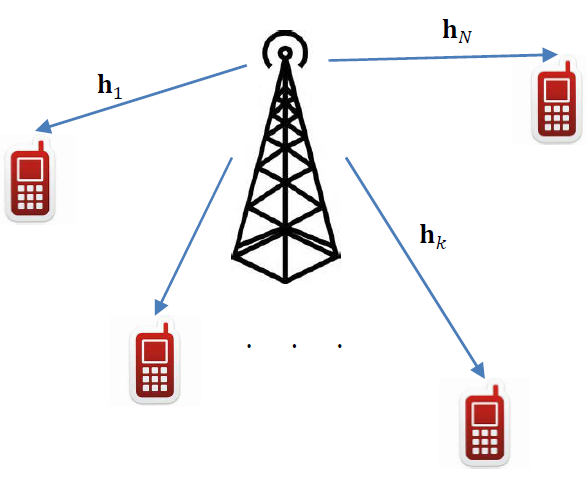
\includegraphics[width=8.8cm]{system.png} % requires the graphicx package
	\caption{Communication scenario}
	\label{fig:system}
\end{figure}
The received signal of Bob $y_b$ is
\begin{eqnarray}
y_b =\mathbf{h}_0^{H}\mathbf{w}_0x_0 + \sum_{k=1}^N \mathbf{h}_{i}^H\mathbf{x}_{i} + n,
\end{eqnarray}
where $x_0$ is the message transmitted from Alice, and $\mathbf{E}\{|x_0|^2\} = 1$; $\mathbf{E}\{\cdot\}$ means expectation; $[\bullet]^H$ means hermitian operation; $\mathbf{w}_{0}$ is a $M \times 1$ vector, which is the beamforming vector of Alice. Alice satisfies the transmit power constraint $\|\mathbf{w}_0\|_2^2 \leq P_0$. $\mathbf{x}_i, i = 1 \cdots N $ are the signals transmitted form Helpers. $\mathbf{x}_i$ is $M$ dimensional  complex Gaussian random vector $\mathbf{x}_i \sim \mathcal{N}(\mathbf{0}, \mathbf{Q}_i)$. $\mathbf{x}_i$ needs to satisfy power constraint $\mathbf{E}\{\|\mathbf{x}_i\|_2^2\}  = \mathrm{Tr}(\mathbf{E}\{\mathbf{x}_i\mathbf{x}_i^H\} )= \mathrm{Tr}(\mathbf{Q}_i) \leq P_i$. 

Assume $n$ is complex Gaussian such that $n \sim \mathcal{N}(0,\sigma_n^2)$. The signal-to-interference-plus-noise ratio of Bob is
\begin{eqnarray}
\mathrm{SINR}_b = \frac{\left| \mathbf{h}_{0}^H\mathbf{w}_{0}\right|^2}{\sigma_n^2 + \sum_{k=1}^{N}\mathbf{h}_{i}^H\mathbf{Q}_{i}\mathbf{h}_i}.
\end{eqnarray}

The received signal of the eavesdropper $y_e$ is
\begin{eqnarray}
y_e = \mathbf{g}_0^H\mathbf{w}_0 + \sum_{i = 1}^N\mathbf{g}_i^H\mathbf{x}_i + m,
\end{eqnarray}
where $\mathbf{g}_0$ is the $M$ dimensional channel vector from Alice to the eavesdropper; $\mathbf{g}_i$ is the $M$ dimensional channel vector from Helper-i to the eavesdropper.   Assume $m$ is complex Gaussian such that $m \sim \mathcal{N}(0,\sigma_m^2)$.
The signal-to-interference-plus-noise ratio of the eavesdropper is
\begin{eqnarray}
\mathrm{SINR}_e &=& \frac{\left| \mathbf{g}_{0}^H\mathbf{w}_{0}\right|^2}{\sigma_m^2 + \sum_{i=1}^{N}\mathbf{g}_{i}^H\mathbf{Q}_{i}\mathbf{g}_i} \label{eq:secure_capacity}.
\end{eqnarray}

The achievable secrecy rate at Bob is given by \cite{6728676}
\begin{equation}
R_s = \log_2\left(1 + \mathrm{SINR}_b\right)-\log_2\left(1 + \mathrm{SINR}_e\right).
\end{equation}


\section{Robust Programming of Secure Communication} \label{sec:robust programming}
Normally the channels to the eavesdroppers are not perfectly known. When the eavesdropper is active \cite{gopala2008secrecy,7015632}, Alice and Helpers can determine the channels. When the eavesdropper is passive, there is a possibility to estimate the channels through the local oscillator power inadvertently leaked from the eavesdropper's receiver radio frequency frontend \cite{mukherjee2012detecting,7015632}. In this paper,  we assume that  Alice and Helpers have imperfect eavesdropper's channels, which is defined as follows. 
\begin{eqnarray}
\mathbf{g}_i = \{\bar{\mathbf{g}}_i + \tilde{\mathbf{g}}_i: \tilde{\mathbf{g}}_i^H \mathbf{R}_i\tilde{\mathbf{g}}_i \leq 1\},\forall i = 0,\cdots, N
\end{eqnarray}
where the positive definite  matrix $\mathbf{R}_i $ defines the variation of channel $\mathbf{g}_i$. 

Helpers use Zero Forcing (ZF) method to transmit noise and eliminate interference to Bob.
The ZF constraint is 
\begin{eqnarray}
\mathbf{h}_i^H\mathbf{x}_i =0 , \forall i = 1,\dots, N\label{eq:ZF_constraint}.
\end{eqnarray}
The ZF constraint can be transformed into the following form
\begin{eqnarray}
&&\mathrm{E}(\|\mathbf{h}_i^H\mathbf{x}_i\|_2^2)\nonumber\\
&=&\mathrm{E}(\mathbf{h}_i^H\mathbf{x}_i\mathbf{x}_i^H\mathbf{h}_i)\nonumber\\
&=&\mathbf{h}_i^H\mathbf{Q}_i \mathbf{h}_i = 0, \forall i = 1,\cdots,N \label{eq:ZF_constraint_relaxed}.
\end{eqnarray}
\subsection{Transmit strategy of Alice}
The basic idea of transmit strategy of the system is to let Alice maximize the signal-to-interference-plus-noise ratio of Bob, and leave the jobs of guaranteeing secure communications to Helpers by generating noise to the eavesdropper.  The signal-to-interference-plus-noise of Bob is 
\begin{eqnarray}
\mathrm{SINR}_b= \frac{\left| \mathbf{h}_{0}^H\mathbf{w}_{0}\right|^2}{\sigma_n^2 }. 
\end{eqnarray}
$\mathrm{SINR}_b$ is not dependent on the transmit covariance matrices of Helpers. The optimal transmission strategy of Alice is Maximum Ratio Transmission (MRT) and the beamforming vector is as follows
\begin{eqnarray}
\mathbf{w}_0 = \sqrt{P_0}\frac{\mathbf{h}_0}{\|\mathbf{h}_0\|_2} \label{eq:optimal_w}.
\end{eqnarray}
And the signal-to-interference-plus-noise ratio of Bob is
\begin{eqnarray} 
\mathrm{SINR}_b= \frac{P_0\| \mathbf{h}_{0}\|_2^2}{\sigma_n^2 }.  \label{eq:SINR_b}
\end{eqnarray}

\subsection{Transmit strategies of Helpers}
The signal-to-interference-plus-noise ratio of the eavesdropper is
\begin{eqnarray}
\mathrm{SINR}_e & < & \frac{\left| \mathbf{g}_{0}^H\mathbf{w}_{0}\right|^2}{\sum_{i=1}^{N}\mathbf{g}_{i}^H\mathbf{Q}_{i}\mathbf{g}_i} \label{eq:neglect_sigma}\\
&=& \frac{|\bar{\mathbf{g}}_0^H\mathbf{w_0} + \tilde{\mathbf{g}}_0^H\mathbf{w}_0|^2}{\sum_{i = 1}^N(\bar{\mathbf{g}}+\tilde{\mathbf{g}}_i)^H\mathbf{Q}_i(\bar{\mathbf{g}}+\tilde{\mathbf{g}}_i)}\\
&\leq & \frac{|\bar{\mathbf{g}}_0^H\mathbf{w_0}|^2 + |\tilde{\mathbf{g}}_0^H\mathbf{w}_0|^2}{\sum_{i = 1}^N(\bar{\mathbf{g}}+\tilde{\mathbf{g}}_i)^H\mathbf{Q}_i(\bar{\mathbf{g}}+\tilde{\mathbf{g}}_i)}\\
&\leq & \frac{|\bar{\mathbf{g}}_0^H\mathbf{w_0}|^2 + \tilde{\mathbf{g}}_0^H\mathbf{w}_0\mathbf{w}_0^H\tilde{\mathbf{g}}_0}{\sum_{i = 1}^N(\bar{\mathbf{g}}+\tilde{\mathbf{g}}_i)^H\mathbf{Q}_i(\bar{\mathbf{g}}+\tilde{\mathbf{g}}_i)}\\
& \leq & \frac{|\bar{\mathbf{g}}_0^H\mathbf{w_0}|^2 + \max(\tilde{\mathbf{g}}_0^H\mathbf{w}_0\mathbf{w}_0^H\tilde{\mathbf{g}}_0)}{\sum_{i = 1}^N(\bar{\mathbf{g}}+\tilde{\mathbf{g}}_i)^H\mathbf{Q}_i(\bar{\mathbf{g}}+\tilde{\mathbf{g}}_i)} .
\label{eq:SINR_e}
\end{eqnarray}
In \eqref{eq:neglect_sigma}, the noise is removed. This is because we consider the case where the eavesdropper has the best receiving performance. We want to limit the maximum signal-to-interference-plus-noise ratio of the eavesdropper within a limit with the imperfect information of the eavesdropper's channels. That is 
\begin{eqnarray}
\max \mathrm{SINR}_e \leq \gamma \label{eq:SINR_constraint},
\end{eqnarray} 
where limit $\gamma$ is the parameter of the proposed algorithm.
And we can guarantee that
\begin{eqnarray}
R_s \geq \log_2\left(1 + P_0\|\mathbf{h}_0\|_2^2/\sigma_n^2\right) - \log_2\left(1 + \gamma\right). \label{eq:secure_capacity1}
\end{eqnarray}
Given the requirement of secrecy rate $R_s$, predefined limit $\gamma$ can be determined from \eqref{eq:secure_capacity1}.

In order to guarantee maximum $\mathrm{SINR}_e$ to be within the predetermined limit $\gamma$, the maximum of the numerator of \eqref{eq:SINR_e} is calculated first by putting \eqref{eq:optimal_w} in \eqref{eq:SINR_e}, and we get the following problem
\begin{equation}\label{eq:numerator problem}
\begin{array}{ll}
\begin{split}
\mathop{\text{maximize}}_{\substack{\{\tilde{\mathbf{g}}_{0}}\}} 
\end{split}  
& \frac{P_0}{\|\mathbf{h}_0\|_2^2}|\bar{\mathbf{g}}_0^H\mathbf{h}_0|^2 +\frac{P_0}{\|\mathbf{h}_0\|_2^2} \tilde{\mathbf{g}}_0^H\mathbf{h}_0\mathbf{h}_0^H\tilde{\mathbf{g}}_0\\
\mathrm{subject~to} &\tilde{\mathbf{g}_0}^H\mathbf{R}_0\tilde{\mathbf{g}}_0 \leq 1.
\end{array}
\end{equation}
Denote $\lambda_{max}(\mathbf{R})$ the largest eigenvalue of matrix $\mathbf{R}$, then
\begin{eqnarray}
\lambda_{max}(\mathbf{R})= \max_{\mathbf{y}^H\mathbf{y} \leq 1} \mathbf{y}^H\mathbf{R}\mathbf{y}.
\end{eqnarray}
Let $\mathbf{R}_0^{1/2}\tilde{\mathbf{g}}_0 = \hat{\mathbf{g}}_0$, the problem of \eqref{eq:numerator problem} is transformed to the following problem
\begin{equation}\label{eq:numerator problem1}
\begin{array}{ll}
\begin{split}
\mathop{\text{maximize}}_{\substack{\{\hat{\mathbf{g}}_{0}}\}} 
\end{split}  
& \frac{P_0}{\|\mathbf{h}_0\|_2^2}|\bar{\mathbf{g}}_0^H\mathbf{h}_0|^2 +\frac{P_0}{\|\mathbf{h}_0\|_2^2} \hat{\mathbf{g}}_0^H\mathbf{R}_0^{-1/2}\mathbf{h}_0\mathbf{h}_0^H\mathbf{R}_0^{-1/2}\hat{\mathbf{g}}_0\\
\mathrm{subject~to} &\hat{\mathbf{g}_0}^H\hat{\mathbf{g}}_0 \leq 1.
\end{array}
\end{equation}

Then the maximum of problem \eqref{eq:numerator problem} is
\begin{eqnarray}
&&\frac{P_0}{\|\mathbf{h}_0\|_2^2}(|\bar{\mathbf{g}}_0^H\mathbf{h}_0|^2 + \lambda_{\mathrm{max}}(\mathbf{R}_0^{-1/2}\mathbf{h}_0\mathbf{h}_0^H\mathbf{R}_0^{-1/2}))\\
&=&\frac{P_0}{\|\mathbf{h}_0\|_2^2}(|\bar{\mathbf{g}}_0^H\mathbf{h}_0|^2 + \|\mathbf{R}_0^{-1/2}\mathbf{h}_0\|_2^2)\label{eq:eigen_norm},
\end{eqnarray} 
where \eqref{eq:eigen_norm} is from the fact that the rank of $\mathbf{R}_0^{-1/2}\mathbf{h}_0$ is 1. Then the constraint of the maximum $\mathrm{SINR}_e$ \eqref{eq:SINR_constraint}  becomes
\begin{eqnarray}
\min_{\tilde{\mathbf{g}}_i: \tilde{\mathbf{g}}_i^H \mathbf{R}_i\tilde{\mathbf{g}}_i \leq 1}\sum_{i=1}^{N}(\bar{\mathbf{g}}+\tilde{\mathbf{g}}_i)^H\mathbf{Q}_i(\bar{\mathbf{g}}+\tilde{\mathbf{g}}_i) \geq \Gamma  \label{eq:artificial noise constraint},
\end{eqnarray}
where $\Gamma =\frac{P_0\left(|\bar{\mathbf{g}}_0^H\mathbf{h}_0|^2 + \|\mathbf{R}_0^{-1/2}\mathbf{h}_0\|_2^2\right)}{\|\mathbf{h}_0\|_2^2\gamma}$ denotes the total minimum interference need to be generated by Helpers to the eavesdropper.

Considering minimizing the transmit power of Helpers as the objective, the problem of secure communications can be formulated as problem $\mathcal{P}_1$ 
\begin{equation}\label{eq:problem1}
(\mathcal{P}_{1}): \begin{array}{ll}
\begin{split}
\mathop{\text{minimize}}_{\substack{\{\mathbf{Q}_{i}}\}} 
\end{split}  
& \sum_{i = 1}^{N}\mathrm{Tr}(\mathbf{Q}_i)\\
\mathrm{subject~to} &\mathrm{Tr}(\mathbf{Q}_i) \leq P_i, \forall i = 1, \cdots, N\\
& \mathbf{h}_i^H \mathbf{Q}_i \mathbf{h}_i= 0, \forall i = 1,\cdots,N\\
&\min_{\tilde{\mathbf{g}}_i: \tilde{\mathbf{g}}_i^H \mathbf{R}_i\tilde{\mathbf{g}}_i \leq 1}\\
&\sum_{i=1}^{N}(\bar{\mathbf{g}}+\tilde{\mathbf{g}}_i)^H\mathbf{Q}_i(\bar{\mathbf{g}}+\tilde{\mathbf{g}}_i) \geq  \Gamma
\end{array}.
\end{equation}
The last constraint of Problem $\mathcal{P}_1$ can be decomposed into $N+1$ constraint by introducing new variables $\{\tau_i\}$, the physical meaning of which are the minimum interferences that Helpers need to generate to Eve. The decomposed constraints are as follows:
\begin{eqnarray}
&\min_{\tilde{\mathbf{g}}_i: \tilde{\mathbf{g}}_i^H \mathbf{R}_i\tilde{\mathbf{g}}_i \leq 1}(\bar{\mathbf{g}}+\tilde{\mathbf{g}}_i)^H\mathbf{Q}_i(\bar{\mathbf{g}}+\tilde{\mathbf{g}}_i) \geq  \tau_i, \forall i = 1,\cdots,N\label{eq:artificial noise constraint decomposed},\nonumber\\
\\
&\sum_{i =1}^{N}\tau_i \geq \Gamma.
\end{eqnarray}
 
 Then Problem $\mathcal{P}_1$ can then be transformed to the following problem
 \begin{equation}\label{eq:problem3}
 (\mathcal{P}_{2}): \begin{array}{ll}
 \begin{split}
 \mathop{\text{minimize}}_{\substack{\{\mathbf{Q}_{i}}\},\{\tau_i\}} 
 \end{split}  
 & \sum_{i = 1}^{N}\mathrm{Tr}(\mathbf{Q}_i)\\
 \mathrm{subject~to} &\mathrm{Tr}(\mathbf{Q}_i) \leq P_i, \forall i = 1, \cdots, N\\
 & \mathbf{h}_i^H \mathbf{Q}_i \mathbf{h}_i= 0, \forall i = 1,\cdots,N\\
 &\min_{\tilde{\mathbf{g}}_i: \tilde{\mathbf{g}}_i^H \mathbf{R}_i\tilde{\mathbf{g}}_i \leq 1}(\bar{\mathbf{g}}+\tilde{\mathbf{g}}_i)^H\mathbf{Q}_i(\bar{\mathbf{g}}+\tilde{\mathbf{g}}_i) \geq  \tau_i. \\
 &\forall i = 1,\cdots,N \nonumber\\
 &\sum_{i =1}^{N}\tau_i \geq \Gamma
 \end{array},
 \end{equation}

The implication of \eqref{eq:artificial noise constraint decomposed} is
\begin{eqnarray}
\tilde{\mathbf{g}}_i^H\mathbf{R}_i\tilde{\mathbf{g}} _i - 1\leq 0  \Rightarrow (\bar{\mathbf{g}}_i+\tilde{\mathbf{g}}_i)^H\mathbf{Q}_i(\bar{\mathbf{g}}_i+\tilde{\mathbf{g}}_i) - \tau_i \geq 0.
\end{eqnarray}
According to the S-Procedure \cite{ConvexOpt_Boyd}, the constraint \eqref{eq:artificial noise constraint decomposed}  in Linear Matrix Inequality (LMI) form is
\begin{eqnarray}
\left[ {\begin{array}{cc}
	\lambda_i\mathbf{R}_i+\mathbf{Q}_i  & \mathbf{Q}_i\bar{\mathbf{g}}_i \\
	\bar{\mathbf{g}}_i^H\mathbf{Q}_i& \bar{\mathbf{g}}_i^H\mathbf{Q}_i\bar{\mathbf{g}} _i- \tau_i -\lambda_i\\
	\end{array} } \right] \succeq \mathbf{0},
\end{eqnarray}
where $\lambda_i \geq 0$ is the introduced new variable. So Problem $\mathcal{P}_2$ can be transformed to Problem $\mathcal{P}_3$
\begin{equation}\label{eq:problem2}
(\mathcal{P}_{3}): \begin{array}{ll}
\begin{split}
\mathop{\text{minimize}}_{\substack{\{\mathbf{Q}_{i}\}, \{\lambda_i\},\{\tau_i\}}} 
\end{split}  
& \sum_{i=1}^N\mathrm{Tr}(\mathbf{Q}_i)\\
\mathrm{subject~to} &\mathrm{Tr}(\mathbf{Q}_i) \leq P_i, \forall i = 1, \cdots, N\\
& \mathbf{h}_i^H\mathbf{Q}_i\mathbf{h}_i= 0,\forall i = 1, \cdots, N\\
&\left[ {\begin{array}{cc}
	\lambda_i\mathbf{R}_i+\mathbf{Q}_i  & \mathbf{Q}_i\bar{\mathbf{g}}_i \\
	\bar{\mathbf{g}}_i^H\mathbf{Q}_i & \bar{\mathbf{g}}_i^H\mathbf{Q}_i\bar{\mathbf{g}}_i - \tau_i -\lambda_i\\
	\end{array} } \right] \\
&\succeq \mathbf{0},\forall i = 1, \cdots, N\\
&\sum_{i=1}^N \tau_i \geq \Gamma
\end{array}.
\end{equation}
Problem $\mathcal{P}_1, \mathcal{P}_2$ and $\mathcal{P}_3$ are equivalent. By solving Problem $\mathcal{P}_3$ using convex optimization tools such as CVX\cite{cvx}, we can solve the secure communications problem.

Based on the solved covariance matrices,  $M$ dimensional noise $\mathbf{x}_i$ can be generated and sent out by Helper-i. The transmitted signal of Helper-i is 
\begin{eqnarray}
\mathbf{x}_i = \mathbf{Q}_i^{1/2}\mathbf{r}_i.
\end{eqnarray} 
$\mathbf{r}_i = [r_{i1},\cdots,r_{iM}]^T$ is Gaussian noise such that $\mathbf{r}_i \sim \mathcal{N}(\mathbf{0},\mathbf{I})$, where $[\bullet]^T$ means transpose operation; $\mathbf{I}$ is $M \times M$ identity matrix. 
The block diagram of the transmitter of Helper-i is shown in Fig.~\ref{fig:transmitter}, where the random generators are independent of each other.
\begin{figure}[h]
	\centering
	\includegraphics[width=8.8cm]{transmitter.png} % requires the graphicx package
	\caption{Block diagram of the transmitter of Helper-i}
	\label{fig:transmitter}
\end{figure}

\section{Distributed algorithm} \label{sec:distributed algorithm}
Solving problem $\mathcal{P}_3$ needs a central unit which collects all the channel information and calculates the covariance matrices of all Helpers. When the number of Helpers is increasing, the centralized algorithm dose not scale well. In this section, we analyze the structure of the problem and propose a distributed algorithm. 

\emph{Proposition 1:} $\{\tau_i^*\}, \{\mathbf{Q}_i^*\}, i = 1, \cdots, N$ are the solution of Problem $\mathcal{P}_2$. If 
\begin{eqnarray}
\frac{\tau_j^*}{\mathrm{Tr}(\mathbf{Q}_j^*)} > \frac{\tau_k^*}{\mathrm{Tr}(\mathbf{Q}_k^*)} \label{eq:efficiency},
\end{eqnarray}
then $\mathrm{Tr}(\mathbf{Q}_j^*) = P_j$.

\emph{Proof:} Assume $\mathrm{Tr}(\mathbf{Q}_j^*) < P_j$. Construct $\tilde{\mathbf{Q}}_j = (1 + \delta) \mathbf{Q}_j^*$ such that $\mathrm{Tr}(\tilde{\mathbf{Q}}_j) = P_j$ and $\tilde{\mathbf{Q}}_k = \frac{\tau_k - \delta\tau_j^*}{\tau_k^*} \mathbf{Q}_k^*$. We have
\begin{eqnarray}
(\bar{\mathbf{g}}_j+\tilde{\mathbf{g}}_j)^H\tilde{\mathbf{Q}}_j(\bar{\mathbf{g}}_j+\tilde{\mathbf{g}}_j)\geq (1+ \delta)\tau_j^*,\\
(\bar{\mathbf{g}}_k+\tilde{\mathbf{g}}_k)^H\tilde{\mathbf{Q}}_k(\bar{\mathbf{g}}_k+\tilde{\mathbf{g}}_k) \geq \tau_k^* - \delta\tau_j^*.
\end{eqnarray}
The same amount interference generated by Help-k and Help-j to the eavesdropper can be guaranteed
\begin{eqnarray}
&&(\bar{\mathbf{g}}_j+\tilde{\mathbf{g}}_j)^H\tilde{\mathbf{Q}}_j(\bar{\mathbf{g}}_j+\tilde{\mathbf{g}}_j) \nonumber\\
&&+ (\bar{\mathbf{g}}_k+\tilde{\mathbf{g}}_k)^H\tilde{\mathbf{Q}}_k(\bar{\mathbf{g}}_k+\tilde{\mathbf{g}}_k)\nonumber\\
&\geq&  \tau_k^* + \tau_j^*,
\end{eqnarray}

So, $\tilde{\mathbf{Q}}_k, \tilde{\mathbf{Q}}_j$ and other $\mathbf{Q}_i^*, i \neq k,j$ satisfy the constraints of Problem $\mathcal{P}_2$. But
\begin{eqnarray}
&&\mathrm{Tr}(\tilde{\mathbf{Q}}_k) + \mathrm{Tr}(\tilde{\mathbf{Q}}_j)\\
&=&\frac{\tau_k^* - \delta\tau_j^*}{\tau_k^*} \mathrm{Tr}(\mathbf{Q}_k^*)  + (1 + \delta)\mathrm{Tr}(\mathbf{Q}_j^*)\\
&=&\mathrm{Tr}(\mathbf{Q}_k^*) + \mathrm{Tr}(\mathbf{Q}_j^*) + \frac{\delta\tau_k^*\mathrm{Tr}(\mathbf{Q}_j^*)-\delta\tau_j^*\mathrm{Tr}(\mathbf{Q}_k^*)}{\tau_k^*}\\
&<&\mathrm{Tr}(\mathbf{Q}_k^*) + \mathrm{Tr}(\mathbf{Q}_j^*) \label{eq:contradiction}
\end{eqnarray}
where \eqref{eq:contradiction} comes from  \eqref{eq:efficiency}.
\eqref{eq:contradiction} means $\tilde{\mathbf{Q}}_k, \tilde{\mathbf{Q}}_j$ and other $\mathbf{Q}_i^*, i \neq k,j$ are the optimal solution of Problem $\mathcal{P}_2$, which is a contradiction.$\blacksquare$

$\frac{\tau_i*}{\mathrm{Tr}(\mathbf{Q}_i^*)}$ defines the interference generated per unit power by Helper-i, and we call it transmit efficiency of Helper-i. Proposition 1 tells that the Helper with higher transmit efficiency should be exploited first until all the transmit power of the Helper is used.


\emph{Proposition 2:} Assume problem \eqref{eq:subproblem1} is feasible when problem parameter $\tau_i = \tau_{i1}$, and the optimal solution is $\mathbf{Q}_i^*$. When the problem parameter $\tau_i = \tau_{i2} \leq \tau_{i1}$, then the optimal solution of the problem is $\frac{\tau_{i2}}{\tau_{i1}}\mathbf{Q}_i^*$ 
\begin{equation}\label{eq:subproblem1}
\begin{array}{ll}
\begin{split}
\mathop{\text{minimize}}_{\substack{\{\mathbf{Q}_{i}}\}} 
\end{split}  
& \mathrm{Tr}(\mathbf{Q}_i)\\
\mathrm{subject~to} &\mathrm{Tr}(\mathbf{Q}_i) \leq P_i\\
& \mathbf{h}_i^H \mathbf{Q}_i \mathbf{h}_i= 0\\
&\min_{\tilde{\mathbf{g}}_i: \tilde{\mathbf{g}}_i^H \mathbf{R}_i\tilde{\mathbf{g}}_i \leq 1}\\
&(\bar{\mathbf{g}}+\tilde{\mathbf{g}}_i)^H\mathbf{Q}_i(\bar{\mathbf{g}}+\tilde{\mathbf{g}}_i) \geq  \tau_{i}
\end{array}.
\end{equation}

\emph{Proof:} Because of the linearity of the constraints of \eqref{eq:subproblem1},  $\frac{\tau_{i2}}{\tau_{i1}}\mathbf{Q}_i^*$ satisfies the all the constraints when $\tau_i = \tau_{i2}$. Assume $\tilde{\mathbf{Q}}_i \neq \frac{\tau_{i2}}{\tau_{i1}}\mathbf{Q}_i^*$ is the optimal value when $\tau_i = \tau_{i2}$ and $\mathrm{Tr}(\tilde{\mathbf{Q}}_i) < \mathrm{Tr}(\frac{\tau_{i2}}{\tau_{i1}}\mathbf{Q}_i^*)$. Then $\frac{\tau_{i1}}{\tau_{i2}}\tilde{\mathbf{Q}}_i$ satisfies all the constraints when $\tau = \tau_{i1}$. But $\frac{\tau_{i1}}{\tau_{i2}}\tilde{\mathbf{Q}}_i \neq \mathbf{Q}_i^*$ and $\mathrm{Tr}(\frac{\tau_{i1}}{\tau_{i2}}\tilde{\mathbf{Q}}_i) < \mathrm{Tr}(\mathbf{Q}_i^*)$ which is a contradiction.$\blacksquare$


Proposition 2 can be interpreted using Fig.~\ref{fig:interpretation of subproblems}. The shaded ellipsoid represents uncertainty of the eavesdropper's channel. When $\mathbf{g}_i$ is in the unshaded ellipsoid, we have $\mathbf{g}_i^H\mathbf{Q}_i\mathbf{g}_i \leq  \tau_{i}$. We want to find the ``biggest" unshaded ellipsoid constrained by the power constraint and ZF constraint, such that the shaded ellipsoid is complete outside of the unshaded ellipsoid. Here the``biggest" ellipsoid corresponds to the $\mathbf{Q}_i$ which has the smallest sum of eigenvalues.  From the figure, we can tell that the shape of the unshaded ellipse is unchanged, but $\mathbf{Q}_i$ is scaled with $\tau_i$.
\begin{figure}[ht]
	\centering
	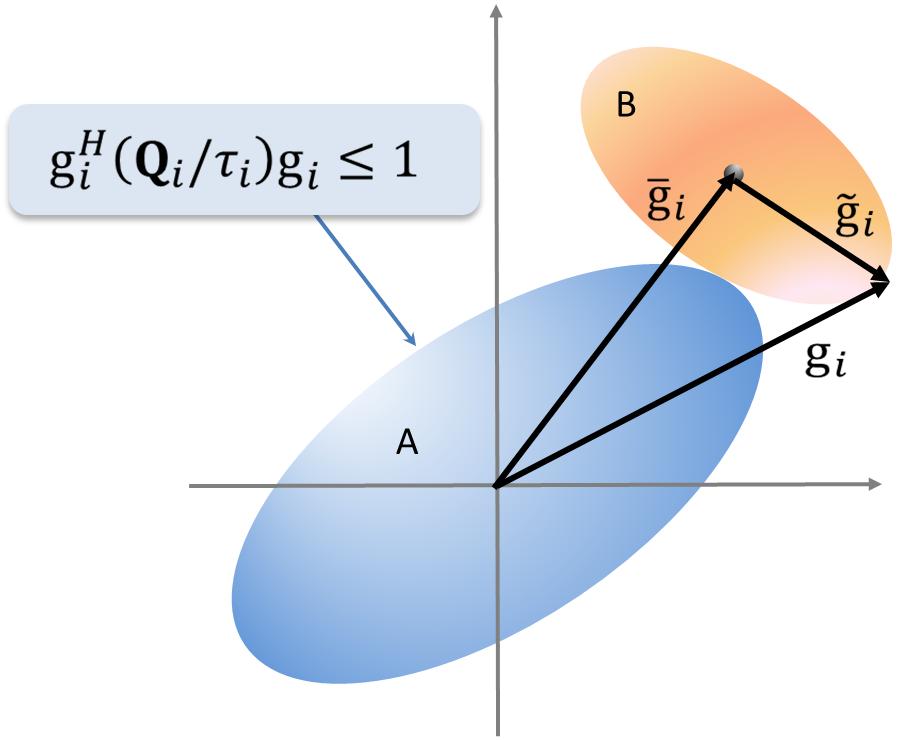
\includegraphics[width=8.8cm]{subproblem.png} % requires the graphicx package
	\caption{Interpretation of subproblems}
	\label{fig:interpretation of subproblems}
\end{figure}
Considering the case where the shaded ellipsoid is enlarged such that it includes the origin, then we cannot find $\mathbf{Q}_i$ to exclude shaded ellipsoid outside any unshaded ellipsoid when $\tau_i$ is positive. That means, if  $\bar{\mathbf{g}}_i^H\mathbf{R}_i\bar{\mathbf{g}}_i \leq 1, \forall i = 1, \cdots,N$, positive interference generated to the eavesdropper cannot be guaranteed, and positive secrecy rate cannot be guaranteed no matter how large the transmit power of the Helpers have.   


Proposition 2 describes the fact that no matter how much interference is needed to be transmitted by each Helper, the transmit covariance is scaled by a real number and the transmit efficiency remains the same.  Based on the fact and Proposition 1, we propose the following algorithm.

\begin{algorithm}
	\caption{}\label{alg:distributed}
	\begin{algorithmic}
		\item[0.] Set $\tau_{\mathrm{min}}$ to a small value. Such as $\tau_{\mathrm{min}} = \Gamma/N$. 
		\item[1.] Each Helper solve \eqref{eq:subproblem1} with $\tau_i = \tau_{\mathrm{min}}$ to get $\mathbf{Q}_i$, and calculate the transmit efficiency $\varepsilon_i = \frac{\tau_{\mathrm{min}}}{\mathrm{Tr}(\mathbf{Q}_i)}$. If problem \eqref{eq:subproblem1} is infeasible, $\varepsilon_i = 0$.
		\item[2.] Broadcast to $\varepsilon_i$ and $\mathrm{Tr}(\mathbf{Q}_i)$ to other Helpers. 
		\item[3.] Each Helper set $\mathcal{E} =\{ {\varepsilon_i,\cdots, \varepsilon_N}\}$ and $\mathcal{I} =\{\}$.
		\item[4.] Each Helper find the maximum transmit efficiency in set $\mathcal{E}$, that is $\varepsilon_i = \max~\mathcal{E}$ (if $\mathcal{E}$ is empty,  the maximum transmit efficiency returned is 0). If $\varepsilon_i = 0$, goto step 7; else $\mathcal{I} := \mathcal{I} + \{i\}$; $\mathcal{E} := \mathcal{E}  - \{\varepsilon_i\}$.
		\item[5.] If $\Gamma \geq \varepsilon_{i} P_i$, $\mathbf{Q}_{i}^* = \frac{P_i}{\mathrm{Tr(\mathrm{Q}}_i)}\mathbf{Q}_i$, $\Gamma := \Gamma - \varepsilon_iP_i$, goto step 4; else $\mathbf{Q}_{i}^* = \frac{\Gamma}{\tau_\mathrm{min}}\mathbf{Q}_i$, go to step 6.
		\item[6.] If $i \in \mathcal{I}$, the transmit covariance of Helper-i is $\mathbf{Q}_i^*$, otherwise the transmit covariance is $\mathbf{0}$.
		\item[7.] There is no solution,  and the required secrecy rate cannot be guaranteed.
	\end{algorithmic}
\end{algorithm}

The basic idea of Algorithm \ref{alg:distributed} is that each Helper calculate the transmit efficiency of generating interference to the eavesdropper and the algorithm always choose the most efficient Helper to generate as much interference as possible. In the algorithm, each Helper solves a convex optimization problem only once distributively, and broadcast the scalar transmit efficiency and the initial transmit power to other Helpers. The network signaling is moderate. After receiving all the information, the most complex work of each Helper is to sort the transmit efficiencies, the complexity of which is $O(N\log(N))$. 


%\section{Simplified Algorithm} \label{sec:simplified algorithm}
%Algorithm \ref{alg: algorithm distributed} is complicated, because every iteration each Helper has to solve a convex optimization problem. Besides, the convergence speed can be quite slow  because of the large range of $\mu$. This sector will propose a simplified algorithm which is easy to implement. 
%
%First we find a projection vector from origin to the set constrained by uncertain area $\mathbf{S}_i$, while satisfying the ZF constraint.
%\begin{equation}\label{eq:projection}
%\begin{array}{ll}
%\begin{split}
%\mathop{\text{minimize}}_{\substack{\mathbf{v}_{i}}} 
%\end{split}  
%& \|\mathbf{w}_i\|_2^2\\
%\mathrm{subject~to}
%& (\mathbf{w}_i-\bar{\mathbf{g}}_i)^H\mathbf{R}_i(\mathbf{w}_i-\bar{\mathbf{g}}_i) \leq 1
%\end{array}
%\end{equation}
%\emph{Proposition 1:} The minimum noise that Helper-i generates to the eavesdropper has the following property
%\begin{eqnarray} \label{eq:simplified interference}
%|\mathbf{g}_i^H\sqrt{p_i}\mathbf{w}_i|^2\geq p_i\|\mathbf{w}_i\|_2^4 \label{eq:simplified interference constraint}
%\end{eqnarray}
%where $p_i \geq 0$ is a scaling factor to control the transmit power of Helper-i. 
%
%\emph{Proof :} 
%Because
%\begin{eqnarray}
%\mathrm{Re}(-\mathbf{w}_i, \mathbf{g}_i - \mathbf{w}_i) \leq 0
%\end{eqnarray},
%we have
%\begin{eqnarray}
%&&\mathrm{Re}(\mathbf{g}_i^H\mathbf{w}_i) \geq \|\mathbf{w_i}\|_2^2\\
%&\Rightarrow&|\mathbf{g}_i^H\mathbf{w}_i| \geq\|\mathbf{w_i}\|_2^2. \blacksquare
%\end{eqnarray}
%
%
%%$\mathbf{w}_i$ define the supporting plane at $\mathbf{w}_i$. Then we find the vector $\mathbf{w}_i$ on the supporting plane which satisfy the ZF condition. $\mathbf{w}_i$ can be got by the following equation which guarantee the minimum norm of $\mathbf{w}_i$
%%\begin{eqnarray}
%%\mathbf{w}_i = \mathbf{A}^H(\mathbf{A}\mathbf{A}^H)^{-1}\mathbf{b}
%%\end{eqnarray}
%%where
%%\begin{equation}\label{eq:A}
%%\mathbf{A}= \left[ {\begin{array}{c}
%%		\mathbf{v}^H\\
%%		\mathbf{h}_i^h\\
%%		\end{array} } \right]
%%\end{equation}
%%and $\mathbf{b_i} = [\|\mathbf{v}_i\|^2;0]^H$
%The projection can be interpreted as Fig.~\ref{fig:projection}.
%\begin{figure}[ht]
%	\centering
%	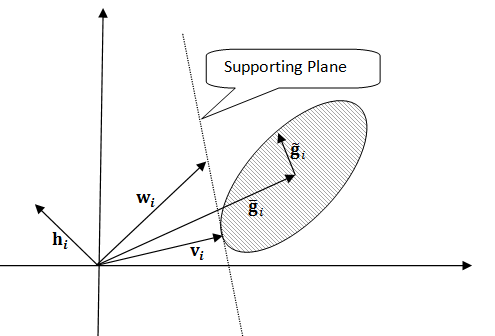
\includegraphics[width=8.8cm]{projection.png} % requires the graphicx package
%	\caption{Interpretation of subproblems}
%	\label{fig:projection}
%\end{figure}.
%
%Each helper transmit using beamforming vector $\sqrt{\rho}_i\mathbf{w}_i$. That is $\mathbf{x}_i = \mathbf{w}_ir_i$ where $r_i \sim \mathcal{N}(0,1)$. So, 
%\begin{eqnarray}
%\mathrm{SINR}_b &=& \frac{P_0\|\mathbf{h}_{0}\|^2}{\sigma_n^2 + \sum_{k=1}^{N}|\mathbf{h}_{i}^H\mathbf{w}_{i}|^2} \\ 
%&=&\frac{\alpha}{\sigma_n^2 + \mathbf{p}^T\mathbf{c}}.
%\end{eqnarray}
%where $\alpha = P_0\|\mathbf{h}_{0}\|^2$.
%\begin{eqnarray}
%	\mathrm{SINR}_e& \geq & \frac{\frac{P_0}{\|\mathbf{h}_0\|_2^2}(|\bar{\mathbf{g}}_0^H\mathbf{h}_0|^2 + \|\mathbf{R}_0^{-1/2}\mathbf{h}_0\|_2^2)}{\sum_{i = 1}^{N}p_i\|\mathbf{w}_i\|^4}\\
%	&=&\frac{\beta}{\mathbf{p}^T\mathbf{d}}
%\end{eqnarray}
%where $\beta = \frac{P_0}{\|\mathbf{h}_0\|_2^2}(|\bar{\mathbf{g}}_0^H\mathbf{h}_0|^2 + \|\mathbf{R}_0^{-1/2}\mathbf{h}_0\|_2^2)$.  And the guaranteed secrecy capacity is
%\begin{eqnarray}
%C_s &=& \log_2(1 + \frac{\alpha}{\sigma_n^2 + \mathbf{p}^T\mathbf{c}}) - \log_2(1 + \frac{\beta}{\mathbf{p}^T\mathbf{d}})\\
%&=&\log_2(\alpha + \sigma_n^2 + \mathbf{p}^T\mathbf{c})-\log_2(\sigma_n^2 + \mathbf{p}^T\mathbf{c}) \nonumber\\
%&&- \log_2(\beta+\mathbf{p}^T\mathbf{d}) + \log_2(\mathbf{p}^T\mathbf{d})
%\end{eqnarray}
%
%For clarity, we give the proposition in \cite{7015632}.
%
%\emph{Proposition 2:} let $a$ is real positive and $ f(a) = -\frac{ab}{\mathrm{ln}2} + \log_2a +\frac{1}{\mathrm{ln}2}$. We have 
%\begin{eqnarray}
%	-log_2b = \max_{a>0}f(a) \label{eq:transformation}
%\end{eqnarray}
%and the optimal solution to the right-hand side of \eqref{eq:transformation} is  $a = 1/b$ \cite{7015632}.
%
%First based on Proposition 2, we transform the guaranteed secrecy capacity to convex form
%\begin{eqnarray}
%C_s = &\log_2(\alpha + \sigma_n^2 +  \mathbf{p}^T\mathbf{c})  + \log_2(\mathbf{p}^T\mathbf{d}) \nonumber\\
%&+ \max_{a_1 > 0}\zeta_1(a_1) +\max_{a_2>0}\zeta_2(a_2) 
%\end{eqnarray}
%where 
%\begin{eqnarray}
%\zeta_1(a_1) = -\frac{a_1}{\mathrm{ln}2}\left( \sigma_n^2 + \mathbf{p}^T\mathbf{c}\right) + \frac{1}{\mathrm{ln}2}\\
%\zeta_2(a_2) = -\frac{a_2}{\mathrm{ln}2}\left(\beta + \mathbf{p}^T\mathbf{d}\right) + \frac{1}{\mathrm{ln}2}
%\end{eqnarray}
%
%
%Similar to the one in the \cite{7015632}, we alternatively optimize $\mathbf{p}$ and $a_i, i = 1,2$. Given the $a_i, i = 1,2$, optimizing $\mathbf{p}$ is equivalent to solving the  following problem to optimize $\mathbf{p}$
%\begin{equation}\label{eq:optimize p}
%\begin{array}{ll}
%\begin{split}
%\mathop{\text{maximize}}_{\substack{\mathbf{p}}} 
%\end{split}  
%& \log(\alpha+\sigma_n^2 + \mathbf{p}^T) + \log(\mathbf{p}^T\mathbf{d}) - a_1\mathbf{p}^T\mathbf{c} - a_2\mathbf{p}^T\mathbf{d}\\
%\mathrm{subject~to}
%& p_i\|\mathbf{w}_i\|_2^2 \leq P_i
%\end{array}
%\end{equation}
%
%Given $\mathbf{p}$, $a_1, a_2$ is given by
%\begin{eqnarray}
%a_1= \frac{1}{\sigma_n^2 + \mathbf{p}^T\mathbf{c}}\\
%a_2= \frac{1}{\beta+\mathbf{p}^T\mathbf{d}}
%\end{eqnarray}
%

%Then the calculated vector $\mathbf{w}_i/\|\mathbf{w}_i\|$ will be used as the beamforming direction of Helper-i. 
%
%\emph{Proposition 1:}  The minimum noise that Helper-i generates to the eavesdropper has the following property
%\begin{eqnarray} \label{eq:simplified interference}
%|\mathbf{g}_i\sqrt{\rho_i}\mathbf{w}_i|^2\geq \rho_i\|\mathbf{v}_i\|_2^4 \label{eq:simplified interference constraint}
%\end{eqnarray}
%where $\rho_i \geq 0$ is a scaling factor to control the transmit power of Helper-i. 
%
%\emph{Proof :} Omitted.
%Because
%\begin{eqnarray}
%\mathrm{Re}(-\mathbf{v}_i, \mathbf{g}_i - \mathbf{v}_i) \leq 0
%\end{eqnarray},
%we have
%\begin{eqnarray}
%&&\mathrm{Re}(\mathbf{g}_i^H\mathbf{v}_i) \geq \|\mathbf{v_i}\|_2^2\\
%&\Rightarrow&|\mathbf{g}_i^H\mathbf{v}_i| \geq\|\mathbf{v_i}\|_2^2
%\end{eqnarray}
%$\mathbf{w}_i$ is in the supporting plane defined by $\mathbf{v}_i$, we have
%\begin{eqnarray}
%\mathbf{w}_i = \mathbf{v}_i + \mathbf{v}_i^{\bot}
%\end{eqnarray}
%Then
%\begin{eqnarray}
%&&|\mathbf{g}_i^H\mathbf{w}_i|\\
%&=&|\mathbf{g}_i^H\mathbf{v}_i+ \mathbf{g}_i^H\mathbf{v}_i^{\bot}|
%\end{eqnarray}
%
%From Proposition 1, Problem $\mathcal{P}_1$ can be transformed to the following easier linear programing problem problem.
% 
%
%\begin{equation}\label{eq:simplified problem}
%\begin{array}{ll}
%\begin{split}
%\mathop{\text{minimize}}_{\substack{\rho_{i}}} 
%\end{split}  
%& \sum_{i =1}^N \rho_i\eta_i\\
%\mathrm{subject~to}
%& 0 \leq \rho_i \eta_i\leq P_i\\
%& \sum_{i = 1}^{N}\rho_i \|\beta_i\|^2 \geq \Gamma
%\end{array}
%\end{equation}
%where $\eta_i = \|\mathbf{w}_i\|_2^2$; $\beta_i = \|\mathbf{v}_i\|_2^2$. And the simplified algorithm is described as Algorithm \ref{alg: algorithm simplified}.
%\begin{algorithm}
%	\caption{}\label{alg: algorithm simplified}
%	\begin{algorithmic}
%		\item[1.] Each Helper solve \eqref{eq:projection} and \eqref{eq:A} to  get $\mathbf{w}_i$, $\eta_i$ and $\beta_i $
%		\item[2.] Broadcast to $\eta_i$  and $\beta_i$ to other Helpers;
%		\item[3.] Each Helper sovle linear programming problem \eqref{eq:simplified problem} and get power allocation $\alpha_i$
%		\item[4.] Each Helper transmit using bearforming vector $\sqrt{\rho_i}\mathbf{w}_i$
%	\end{algorithmic}
%\end{algorithm}
%
%Compared to the distributed algorithm proposed in Section \ref{sec:robust programming}, the simplified algorithm does not need to solve complex convex optimization problem every iteration. Each Help only calculate the beamforming vector at the beginning of the algorithm, and the power allocation of the beamforming vectors is then directly determined in the central unit or distributively. The iterative process is avoided. Besides,  simplified algorithm uses beamforming method other than precoding method, which also simplify the implementation.

\section{Numerical Results} \label{sec:numerical results}
A radio network like Fig. ~\ref{fig:system} is simulated. Alice and Helpers have four transmit antennas, which is $M_{Ts}= 4$. The channel from Alice to Bob is randomly selected and normalized, which means $\|\mathbf{h}_0\| = 1$. The channel between Helpers and Bob are randomly generated such that $\|\mathbf{h}_i\| = \alpha$.  The average channels among Alice, Helpers  and Eve are randomly generated such that $\|\bar{\mathbf{g}}_i\| = \alpha$. $\alpha$ is a random variable, which is used to simulated the random distance of Alice, Bob, Helpers and Eve relative to each other. $\alpha \in  [0.1,10]$ is uniformly distributed.  Positive hermitian matrix $\mathbf{R}_i$ is randomly generated, and $\|\mathbf{R}_i\|_F = s$. $s$ defines the greatness of the eavesdropper's channel uncertainty. The larger $s$ is, the smaller channel uncertainty is. 
For simplicity, we assume Alice and all Helpers have the same transmit power. That is $P_0=P_i = P$. The noise variance of Bob is normalize to 1,  and according to \eqref{eq:SINR_b} , we have $\mathrm{SINR}_b = P$. In the simulations, we set $\mathrm{SNR}_b = 20 \mathrm{dB}$, which means $P = 100$.


\begin{figure}[!ht]
	\centering
	\includegraphics[width=8.8cm]{Changing_Cs.eps} % requires the graphicx package
	\caption{Relationship of total transmit power with required secrecy rates.}
	\label{fig:Changing_Cs}
\end{figure}

Fig.~\ref{fig:Changing_Cs} shows the total transmit transmit power of Helpers. In this simulation, we fix the simulation parameter $s = 1$. When there are more Helpers, the total transmit power is lower. It is because that there are more strategies for Helpers to choose to generate noise. When the requirement of secrecy rate is higher, we need more total transmit power to generate enough noise to the eavesdropper. Under the setting of simulation, compared to the transmit power limit of each Helper, the actual total transmit power of Helpers is small. It means on average, Helpers only need small transmit power to generate noise to the eavesdropper.

\begin{figure}[!ht]
	\centering
	\includegraphics[width=8.8cm]{Changing_s.eps} % requires the graphicx package
	\caption{Relationship of total transmit power with the simulation parameter $s$.}
	\label{fig:Changing_s}
\end{figure}

Fig.~\ref{fig:Changing_s} shows the total transmit power of Helpers with changing simulation parameter $s$. In this simulation, we fix the secrecy rate requirement $R_s \geq 3 $ b/s/Hz. The figure shows that when s is small, which means the uncertainty is great, Helpers need more power to transmit noise to realize secure communications. It is because that when the uncertainty is greater, Helpers need to transmit more noise to make sure that the performance of the eavesdropper can be degraded enough to guarantee the secrecy rate for all the possible eavesdropper's channels.

\begin{figure}[!ht]
	\centering
	\includegraphics[width=8.8cm]{Cs_success.eps} % requires the graphicx package
	\caption{Relationship of successfully realizing secure communications with required secrecy rates.}
	\label{fig:Cs_success}
\end{figure}
\begin{figure}[!ht]
	\centering
	\includegraphics[width=8.8cm]{s_success.eps} % requires the graphicx package
	\caption{Relationship of successfully realizing secure communications with the simulation parameter $s$.}
	\label{fig:s_success}
\end{figure}

It is possible that with the aid of Helpers the system still cannot realize the required secure communications. Fig.~\ref{fig:Cs_success} and Fig.~\ref{fig:s_success} show the relationship of successfully realizing the required secure communications with the secrecy rate requirement and the eavesdropper's channel uncertainty. For Fig.~\ref{fig:Cs_success}, we fix the simulation parameter $s = 1$. For Fig.~\ref{fig:s_success} we fix the required secrecy rate $R_s \geq 3$ b/s/Hz. It can be shown that higher secrecy rate requirement and greater channel uncertainty will cause less success of secure communications. But by increasing the number of Helpers and using the distributed algorithm proposed in Section \ref{sec:distributed algorithm} which scales well with increasing number of Helpers, we can increase the rate of success of secure communications easily. 

% An example of a floating figure using the graphicx package.
% Note that \label must occur AFTER (or within) \caption.
% For figures, \caption should occur after the \includegraphics.
% Note that IEEEtran v1.7 and later has special internal code that
% is designed to preserve the operation of \label within \caption
% even when the captionsoff option is in effect. However, because
% of issues like this, it may be the safest practice to put all your
% \label just after \caption rather than within \caption{}.
%
% Reminder: the "draftcls" or "draftclsnofoot", not "draft", class
% option should be used if it is desired that the figures are to be
% displayed while in draft mode.
%
%\begin{figure}[!t]
%\centering
%\includegraphics[width=2.5in]{myfigure}
% where an .eps filename suffix will be assumed under latex, 
% and a .pdf suffix will be assumed for pdflatex; or what has been declared
% via \DeclareGraphicsExtensions.
%\caption{Simulation results for the network.}
%\label{fig_sim}
%\end{figure}

% Note that IEEE typically puts floats only at the top, even when this
% results in a large percentage of a column being occupied by floats.


% An example of a double column floating figure using two subfigures.
% (The subfig.sty package must be loaded for this to work.)
% The subfigure \label commands are set within each subfloat command,
% and the \label for the overall figure must come after \caption.
% \hfil is used as a separator to get equal spacing.
% Watch out that the combined width of all the subfigures on a 
% line do not exceed the text width or a line break will occur.
%
%\begin{figure*}[!t]
%\centering
%\subfloat[Case I]{\includegraphics[width=2.5in]{box}%
%\label{fig_first_case}}
%\hfil
%\subfloat[Case II]{\includegraphics[width=2.5in]{box}%
%\label{fig_second_case}}
%\caption{Simulation results for the network.}
%\label{fig_sim}
%\end{figure*}
%
% Note that often IEEE papers with subfigures do not employ subfigure
% captions (using the optional argument to \subfloat[]), but instead will
% reference/describe all of them (a), (b), etc., within the main caption.
% Be aware that for subfig.sty to generate the (a), (b), etc., subfigure
% labels, the optional argument to \subfloat must be present. If a
% subcaption is not desired, just leave its contents blank,
% e.g., \subfloat[].


% An example of a floating table. Note that, for IEEE style tables, the
% \caption command should come BEFORE the table and, given that table
% captions serve much like titles, are usually capitalized except for words
% such as a, an, and, as, at, but, by, for, in, nor, of, on, or, the, to
% and up, which are usually not capitalized unless they are the first or
% last word of the caption. Table text will default to \footnotesize as
% IEEE normally uses this smaller font for tables.
% The \label must come after \caption as always.
%
%\begin{table}[!t]
%% increase table row spacing, adjust to taste
%\renewcommand{\arraystretch}{1.3}
% if using array.sty, it might be a good idea to tweak the value of
% \extrarowheight as needed to properly center the text within the cells
%\caption{An Example of a Table}
%\label{table_example}
%\centering
%% Some packages, such as MDW tools, offer better commands for making tables
%% than the plain LaTeX2e tabular which is used here.
%\begin{tabular}{|c||c|}
%\hline
%One & Two\\
%\hline
%Three & Four\\
%\hline
%\end{tabular}
%\end{table}


% Note that the IEEE does not put floats in the very first column
% - or typically anywhere on the first page for that matter. Also,
% in-text middle ("here") positioning is typically not used, but it
% is allowed and encouraged for Computer Society conferences (but
% not Computer Society journals). Most IEEE journals/conferences use
% top floats exclusively. 
% Note that, LaTeX2e, unlike IEEE journals/conferences, places
% footnotes above bottom floats. This can be corrected via the
% \fnbelowfloat command of the stfloats package.




\section{Conclusion} \label{sec:conclusion}
This paper discusses a method to implement secure communications. The channels from the intended transmitter and Helpers are known. But the channels to the eavesdropper are imperfectly known. The intended transmitter uses MRT to maximize the signal-to-interference-plus-noise ratio of the intended receiver. Helpers transmit noise to degrade the performance of the eavesdropper to guarantee the required secrecy rate. The structure of the transmitted noise is exploited and the transmit strategies of Helpers are formulate as a robust programming problem, in which the transmit covariance matrices are the optimization variable. Based on the solved transmit covariances of Helpers, secure communications can be implemented. In order to ease the implementation of secure communications, a distributed algorithm, which scales well with increasing number of Helpers, is proposed. Simulation results show that with the aiding of Helpers, robust secure communications can be realized.




% conference papers do not normally have an appendix


% use section* for acknowledgment
%\section*{Acknowledgment}


%The authors would like to thank...





% trigger a \newpage just before the given reference
% number - used to balance the columns on the last page
% adjust value as needed - may need to be readjusted if
% the document is modified later
%\IEEEtriggeratref{8}
% The "triggered" command can be changed if desired:
%\IEEEtriggercmd{\enlargethispage{-5in}}

% references section

% can use a bibliography generated by BibTeX as a .bbl file
% BibTeX documentation can be easily obtained at:
% http://www.ctan.org/tex-archive/biblio/bibtex/contrib/doc/
% The IEEEtran BibTeX style support page is at:
% http://www.michaelshell.org/tex/ieeetran/bibtex/
%\bibliographystyle{IEEEtran}
% argument is your BibTeX string definitions and bibliography database(s)
%\bibliography{IEEEabrv,../bib/paper}
%
% <OR> manually copy in the resultant .bbl file
% set second argument of \begin to the number of references
% (used to reserve space for the reference number labels box)
%\begin{thebibliography}{1}
\bibliographystyle{IEEEtran}
\bibliography{IEEEabrv,PHY}
%\end{thebibliography}




% that's all folks
\end{document}


